% !TEX TS-program = pdflatex
% !TEX encoding = UTF-8 Unicode

% This is a simple template for a LaTeX document using the "article" class.
% See "book", "report", "letter" for other types of document.

\documentclass[11pt]{article} % use larger type; default would be 10pt

\usepackage[utf8]{inputenc} % set input encoding (not needed with XeLaTeX)

%%% Examples of Article customizations
% These packages are optional, depending whether you want the features they provide.
% See the LaTeX Companion or other references for full information.

%%% PAGE DIMENSIONS
\usepackage{geometry} % to change the page dimensions
\usepackage{graphicx}
\geometry{a4paper} % or letterpaper (US) or a5paper or....
% \geometry{margin=2in} % for example, change the margins to 2 inches all round
% \geometry{landscape} % set up the page for landscape
%   read geometry.pdf for detailed page layout information

\usepackage{graphicx} % support the \includegraphics command and options

% \usepackage[parfill]{parskip} % Activate to begin paragraphs with an empty line rather than an indent

%%% PACKAGES
\usepackage{booktabs} % for much better looking tables
\usepackage{array} % for better arrays (eg matrices) in maths
\usepackage{paralist} % very flexible & customisable lists (eg. enumerate/itemize, etc.)
\usepackage{verbatim} % adds environment for commenting out blocks of text & for better verbatim
\usepackage{subfig} % make it possible to include more than one captioned figure/table in a single float
% These packages are all incorporated in the memoir class to one degree or another...

%%% HEADERS & FOOTERS
\usepackage{fancyhdr} % This should be set AFTER setting up the page geometry
\pagestyle{fancy} % options: empty , plain , fancy
%\setlength{\headheight}{-25pt}
\renewcommand{\headrulewidth}{0pt} % customise the layout...
\lhead{}\chead{}\rhead{}
\lfoot{}\cfoot{\thepage}\rfoot{}

%%% SECTION TITLE APPEARANCE
\usepackage{sectsty}
\allsectionsfont{\sffamily\mdseries\upshape} % (See the fntguide.pdf for font help)
% (This matches ConTeXt defaults)

%%% ToC (table of contents) APPEARANCE
\usepackage[nottoc,notlof,notlot]{tocbibind} % Put the bibliography in the ToC
\usepackage[titles,subfigure]{tocloft} % Alter the style of the Table of Contents
\renewcommand{\cftsecfont}{\rmfamily\mdseries\upshape}
\renewcommand{\cftsecpagefont}{\rmfamily\mdseries\upshape} % No bold!

%%% END Article customizations

%%% The "real" document content comes below...

\title{Homework 1}
\author{Maksim Levental}
%\date{} % Activate to display a given date or no date (if empty),
         % otherwise the current date is printed 

\usepackage{listings}
\usepackage{color}

\definecolor{dkgreen}{rgb}{0,0.6,0}
\definecolor{gray}{rgb}{0.5,0.5,0.5}
\definecolor{mauve}{rgb}{0.58,0,0.82}

\lstset{frame=tb,
  language=C++,
  aboveskip=3mm,
  belowskip=3mm,
  showstringspaces=false,
  columns=flexible,
  basicstyle={\small\ttfamily},
  numbers=none,
  numberstyle=\tiny\color{gray},
  keywordstyle=\color{blue},
  commentstyle=\color{dkgreen},
  stringstyle=\color{mauve},
  breaklines=false,
  breakatwhitespace=false,
  tabsize=3,
  frame=0
}

\begin{document}
\maketitle

\section*{Problem 1}

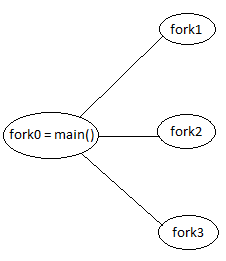
\includegraphics{problem1.png}

\section*{Problem 2}

\begin{lstlisting}
#include <stdlib.h>
#include <stdio.h>
#include <string.h>
#include <unistd.h>

int main(int argc, char *argv[])
{

	int fd[2][2];
	
	if(pipe(fd[0]) == -1){ perror("pipe error"); return(1); }
	if(pipe(fd[1]) == -1){ perror("pipe error"); return(1); }
	
	dup2(fd[0][0], STDIN_FILENO);
	//parent doesn't write to pipe 1, only reads, so this end is closed
	close(fd[0][1]);
	dup2(fd[1][1], STDOUT_FILENO);
	//parent doesn't read from pipe 2, only writes, so this end is closed
	close(fd[1][0]);

	char buf[80], *p;
	p = fgets (buf, 80, stdin); //parent reads from std_in, which is aliased to read end of pipe 1
	printf("s", p); //parents writes to std_out, which is aliased to write end of pipe 2
	      
	if(fork() == 0){	     
		//child writes to write end of first pipe, parent reads from read end
	 	dup2(fd[0][1], STDOUT_FILENO);
		//read end of first pipe is closed because this child doesn't read from from first pipe
	 	close(fd[0][0]);
		//both ends of pipe 2 are closed because this child doesn't use pipe 2 at all
		close(fd[1][0]);
		close(fd[1][1]);

		printf("hello to fork 2!"); //fork 1 writes to std_out, which is read by parent
	}
	  
	if(fork() == 0){
		//child reads from read end of second pipe, parent writes to write end of second pipe
		dup2(fd[1][0], STDIN_FILENO);
		//write end of first pipe is closed because this child doesn't write
		close(fd[1][1]);
		//both ends of pipe 1 are closed because this child doesn't use pipe 1 at all
		close(fd[0][0]);
		close(fd[0][1]);

		char buf[80], *p;
		p = fgets (buf, 80, stdin); //fork 2 reads from std_in, which is written to by parent
		

	}
	  
	wait(0);
	wait(0);

}
\end{lstlisting}

\section*{Problem 3}

Typing a URL into a web browser and hitting enter (\textbf{a}) would definitely result in a system call, if not several. System calls would need to be made to open sockets if they're not open (closed due to idleness if previously opened) to the servers and intermediaries that connect the computer to that site. This would require access to the Network Interface Card or WiFi card.

Playing an MP3 song on a media player (\textbf{b}) would certainly result in system calls. Firstly to data storage to fetch the song to be played and then audio hardware to play the songs through the speakers.

Compiling Java source (\textbf{c}) would  result in system calls because disk management hardware is being used, to load the actual source into the compiler from the source file on disk, and to save the compiled executable files.

Terminating an application by pressing the X button on the window (\textbf{d}) might result in system calls to kill thread associated with the application, depending on what kind of thread management scheme is implemented in the particular OS the program is running on.

\section*{Problem 4}

\subsection*{a.}

A TRAP instruction is a software interrupt produced by the a process in user mode. It is used to initiate a processor operating context switch to kernel mode. 

\subsection*{b.}

A TRAP instruction can be executed in user-mode. For example in UNIX there is a command called trap which takes a numerical argument and requests a privileged instruction execution.

\subsection*{c.}

Some typical parameters are exit, read, write, seek, close, and they're stored in register R0.

\section*{Problem 5}

\subsection*{a.}

The operating system stores process information in a data structure called the Process Control Block. They typically have members and fields classified into 3 types: Identification data, state data, and control data. Stored in the PCB are things like current state (ready, blocked, running), the process ID (corresponding to an index in the process control table discussed in part \textbf{c}), the parent process if there is one, the current state of the PC counter, the processes' address space, the current CPU status word, etc.

\subsection*{b.}

The operating system needs to have fast access to the PCB because it needs to be able to cary out context switches between running processes seemlessly, and context switches involve loading the stored address space of the sleeping process back into physical memory.

\subsection*{c.}

The operating system makes sure it has fast access to the PCB of each process by storing pointers to them in the process table. The pointer to a process with a PCB is the processid field stored in the PCB itself.

\subsection*{d.}

The operating systems needs to store process information because it is the way in which multitasking is in fact implemented. It needs this information in order to be able to context switch and run multiple processes without restarting their execution flow all the way from the beginning. 

\end{document}
